% This file was created with tikzplotlib v0.10.1.
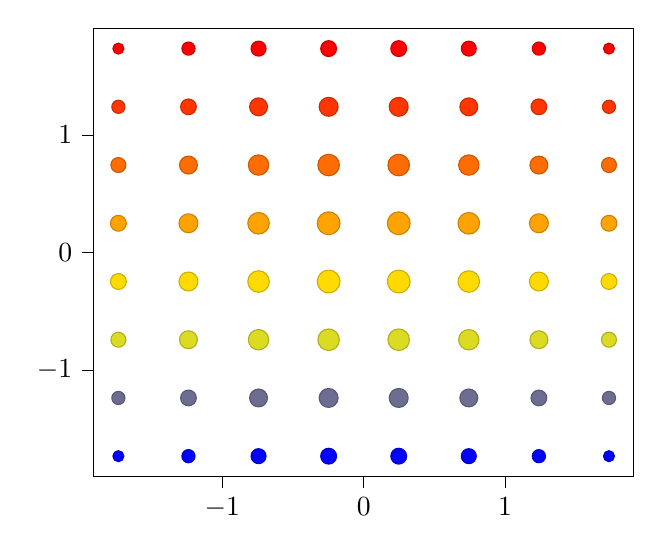
\begin{tikzpicture}

\definecolor{darkgray176}{RGB}{176,176,176}
\definecolor{steelblue31119180}{RGB}{31,119,180}

\begin{axis}[
tick align=outside,
tick pos=left,
x grid style={darkgray176},
xmin=-1.90730187892914, xmax=1.90730187892914,
xtick style={color=black},
y grid style={darkgray176},
ymin=-1.90730187892914, ymax=1.90730187892914,
ytick style={color=black}
]
\addplot [
  draw=steelblue31119180,
  fill=steelblue31119180,
  mark=*,
  only marks,
  scatter,
  scatter/@pre marker code/.append style={/tikz/mark size=\perpointmarksize},
  visualization depends on={\thisrow{sizedata} \as\perpointmarksize}
]
table{%
x  y  sizedata
-1.73391079902649 1.73391079902649 1.9902518
-1.23850774765015 1.73391079902649 2.3760042
-0.743104636669159 1.73391079902649 2.7039983
-0.247701555490494 1.73391079902649 2.8618598
0.247701555490494 1.73391079902649 2.8618598
0.743104636669159 1.73391079902649 2.7039983
1.23850774765015 1.73391079902649 2.3760042
1.73391079902649 1.73391079902649 1.9902518
-1.73391079902649 1.23850774765015 2.3760042
-1.23850774765015 1.23850774765015 2.8365235
-0.743104636669159 1.23850774765015 3.2280898
-0.247701555490494 1.23850774765015 3.416548
0.247701555490494 1.23850774765015 3.416548
0.743104636669159 1.23850774765015 3.2280898
1.23850774765015 1.23850774765015 2.8365235
1.73391079902649 1.23850774765015 2.3760042
-1.73391079902649 0.743104636669159 2.7039983
-1.23850774765015 0.743104636669159 3.2280898
-0.743104636669159 0.743104636669159 3.6737092
-0.247701555490494 0.743104636669159 3.8881829
0.247701555490494 0.743104636669159 3.8881829
0.743104636669159 0.743104636669159 3.6737092
1.23850774765015 0.743104636669159 3.2280898
1.73391079902649 0.743104636669159 2.7039983
-1.73391079902649 0.247701555490494 2.8618598
-1.23850774765015 0.247701555490494 3.416548
-0.743104636669159 0.247701555490494 3.8881829
-0.247701555490494 0.247701555490494 4.115178
0.247701555490494 0.247701555490494 4.115178
0.743104636669159 0.247701555490494 3.8881829
1.23850774765015 0.247701555490494 3.416548
1.73391079902649 0.247701555490494 2.8618598
-1.73391079902649 -0.247701555490494 2.8618598
-1.23850774765015 -0.247701555490494 3.416548
-0.743104636669159 -0.247701555490494 3.8881829
-0.247701555490494 -0.247701555490494 4.115178
0.247701555490494 -0.247701555490494 4.115178
0.743104636669159 -0.247701555490494 3.8881829
1.23850774765015 -0.247701555490494 3.416548
1.73391079902649 -0.247701555490494 2.8618598
-1.73391079902649 -0.743104636669159 2.7039983
-1.23850774765015 -0.743104636669159 3.2280898
-0.743104636669159 -0.743104636669159 3.6737092
-0.247701555490494 -0.743104636669159 3.8881829
0.247701555490494 -0.743104636669159 3.8881829
0.743104636669159 -0.743104636669159 3.6737092
1.23850774765015 -0.743104636669159 3.2280898
1.73391079902649 -0.743104636669159 2.7039983
-1.73391079902649 -1.23850774765015 2.3760042
-1.23850774765015 -1.23850774765015 2.8365235
-0.743104636669159 -1.23850774765015 3.2280898
-0.247701555490494 -1.23850774765015 3.416548
0.247701555490494 -1.23850774765015 3.416548
0.743104636669159 -1.23850774765015 3.2280898
1.23850774765015 -1.23850774765015 2.8365235
1.73391079902649 -1.23850774765015 2.3760042
-1.73391079902649 -1.73391079902649 1.9902518
-1.23850774765015 -1.73391079902649 2.3760042
-0.743104636669159 -1.73391079902649 2.7039983
-0.247701555490494 -1.73391079902649 2.8618598
0.247701555490494 -1.73391079902649 2.8618598
0.743104636669159 -1.73391079902649 2.7039983
1.23850774765015 -1.73391079902649 2.3760042
1.73391079902649 -1.73391079902649 1.9902518
};
\end{axis}

\end{tikzpicture}
